\documentclass[twoside]{book}

% Packages required by doxygen
\usepackage{fixltx2e}
\usepackage{calc}
\usepackage{doxygen}
\usepackage[export]{adjustbox} % also loads graphicx
\usepackage{graphicx}
\usepackage[utf8]{inputenc}
\usepackage{makeidx}
\usepackage{multicol}
\usepackage{multirow}
\PassOptionsToPackage{warn}{textcomp}
\usepackage{textcomp}
\usepackage[nointegrals]{wasysym}
\usepackage[table]{xcolor}

% Font selection
\usepackage[T1]{fontenc}
\usepackage[scaled=.90]{helvet}
\usepackage{courier}
\usepackage{amssymb}
\usepackage{sectsty}
\renewcommand{\familydefault}{\sfdefault}
\allsectionsfont{%
  \fontseries{bc}\selectfont%
  \color{darkgray}%
}
\renewcommand{\DoxyLabelFont}{%
  \fontseries{bc}\selectfont%
  \color{darkgray}%
}
\newcommand{\+}{\discretionary{\mbox{\scriptsize$\hookleftarrow$}}{}{}}

% Page & text layout
\usepackage{geometry}
\geometry{%
  a4paper,%
  top=2.5cm,%
  bottom=2.5cm,%
  left=2.5cm,%
  right=2.5cm%
}
\tolerance=750
\hfuzz=15pt
\hbadness=750
\setlength{\emergencystretch}{15pt}
\setlength{\parindent}{0cm}
\setlength{\parskip}{3ex plus 2ex minus 2ex}
\makeatletter
\renewcommand{\paragraph}{%
  \@startsection{paragraph}{4}{0ex}{-1.0ex}{1.0ex}{%
    \normalfont\normalsize\bfseries\SS@parafont%
  }%
}
\renewcommand{\subparagraph}{%
  \@startsection{subparagraph}{5}{0ex}{-1.0ex}{1.0ex}{%
    \normalfont\normalsize\bfseries\SS@subparafont%
  }%
}
\makeatother

% Headers & footers
\usepackage{fancyhdr}
\pagestyle{fancyplain}
\fancyhead[LE]{\fancyplain{}{\bfseries\thepage}}
\fancyhead[CE]{\fancyplain{}{}}
\fancyhead[RE]{\fancyplain{}{\bfseries\leftmark}}
\fancyhead[LO]{\fancyplain{}{\bfseries\rightmark}}
\fancyhead[CO]{\fancyplain{}{}}
\fancyhead[RO]{\fancyplain{}{\bfseries\thepage}}
\fancyfoot[LE]{\fancyplain{}{}}
\fancyfoot[CE]{\fancyplain{}{}}
\fancyfoot[RE]{\fancyplain{}{\bfseries\scriptsize Generated by Doxygen }}
\fancyfoot[LO]{\fancyplain{}{\bfseries\scriptsize Generated by Doxygen }}
\fancyfoot[CO]{\fancyplain{}{}}
\fancyfoot[RO]{\fancyplain{}{}}
\renewcommand{\footrulewidth}{0.4pt}
\renewcommand{\chaptermark}[1]{%
  \markboth{#1}{}%
}
\renewcommand{\sectionmark}[1]{%
  \markright{\thesection\ #1}%
}

% Indices & bibliography
\usepackage{natbib}
\usepackage[titles]{tocloft}
\setcounter{tocdepth}{3}
\setcounter{secnumdepth}{5}
\makeindex

% Hyperlinks (required, but should be loaded last)
\usepackage{ifpdf}
\ifpdf
  \usepackage[pdftex,pagebackref=true]{hyperref}
\else
  \usepackage[ps2pdf,pagebackref=true]{hyperref}
\fi
\hypersetup{%
  colorlinks=true,%
  linkcolor=blue,%
  citecolor=blue,%
  unicode%
}

% Custom commands
\newcommand{\clearemptydoublepage}{%
  \newpage{\pagestyle{empty}\cleardoublepage}%
}

\usepackage{caption}
\captionsetup{labelsep=space,justification=centering,font={bf},singlelinecheck=off,skip=4pt,position=top}

%===== C O N T E N T S =====

\begin{document}

% Titlepage & ToC
\hypersetup{pageanchor=false,
             bookmarksnumbered=true,
             pdfencoding=unicode
            }
\pagenumbering{alph}
\begin{titlepage}
\vspace*{7cm}
\begin{center}%
{\Large m\+Lego \\[1ex]\large 1.\+1 }\\
\vspace*{1cm}
{\large Generated by Doxygen 1.8.13}\\
\end{center}
\end{titlepage}
\clearemptydoublepage
\pagenumbering{roman}
\tableofcontents
\clearemptydoublepage
\pagenumbering{arabic}
\hypersetup{pageanchor=true}

%--- Begin generated contents ---
\chapter{Class Index}
\section{Class List}
Here are the classes, structs, unions and interfaces with brief descriptions\+:\begin{DoxyCompactList}
\item\contentsline{section}{\hyperlink{class_barre}{Barre} \\*The \hyperlink{class_barre}{Barre} class }{\pageref{class_barre}}{}
\item\contentsline{section}{\hyperlink{class_barre_carre}{Barre\+Carre} \\*The \hyperlink{class_barre_carre}{Barre\+Carre} class }{\pageref{class_barre_carre}}{}
\item\contentsline{section}{\hyperlink{class_barre_rectangle}{Barre\+Rectangle} \\*The \hyperlink{class_barre_rectangle}{Barre\+Rectangle} class }{\pageref{class_barre_rectangle}}{}
\item\contentsline{section}{\hyperlink{class_barre_ronde}{Barre\+Ronde} \\*The \hyperlink{class_barre_ronde}{Barre\+Ronde} class }{\pageref{class_barre_ronde}}{}
\end{DoxyCompactList}

\chapter{File Index}
\section{File List}
Here is a list of all files with brief descriptions\+:\begin{DoxyCompactList}
\item\contentsline{section}{\hyperlink{barre_8cpp}{barre.\+cpp} }{\pageref{barre_8cpp}}{}
\item\contentsline{section}{\hyperlink{barre_8h}{barre.\+h} }{\pageref{barre_8h}}{}
\item\contentsline{section}{\hyperlink{barrecarre_8cpp}{barrecarre.\+cpp} }{\pageref{barrecarre_8cpp}}{}
\item\contentsline{section}{\hyperlink{barrecarre_8h}{barrecarre.\+h} }{\pageref{barrecarre_8h}}{}
\item\contentsline{section}{\hyperlink{barrerectangle_8cpp}{barrerectangle.\+cpp} }{\pageref{barrerectangle_8cpp}}{}
\item\contentsline{section}{\hyperlink{barrerectangle_8h}{barrerectangle.\+h} }{\pageref{barrerectangle_8h}}{}
\item\contentsline{section}{\hyperlink{barreronde_8cpp}{barreronde.\+cpp} }{\pageref{barreronde_8cpp}}{}
\item\contentsline{section}{\hyperlink{barreronde_8h}{barreronde.\+h} }{\pageref{barreronde_8h}}{}
\item\contentsline{section}{\hyperlink{main_8cpp}{main.\+cpp} }{\pageref{main_8cpp}}{}
\end{DoxyCompactList}

\chapter{Class Documentation}
\hypertarget{class_barre}{}\section{Barre Class Reference}
\label{class_barre}\index{Barre@{Barre}}


The \hyperlink{class_barre}{Barre} class.  




{\ttfamily \#include $<$barre.\+h$>$}

\subsection*{Public Member Functions}
\begin{DoxyCompactItemize}
\item 
\hyperlink{class_barre_ac9742650be9a059e9291e6850c827b7a}{Barre} (string \+\_\+reference, const unsigned int \+\_\+longueur, const double \+\_\+densite, string \+\_\+nom\+Alliage)
\begin{DoxyCompactList}\small\item\em \hyperlink{class_barre_ac9742650be9a059e9291e6850c827b7a}{Barre\+::\+Barre}. \end{DoxyCompactList}\item 
void \hyperlink{class_barre_aead6bcfe08b3a9727ffc1e9a236937a9}{Afficher\+Caracteristique} ()
\begin{DoxyCompactList}\small\item\em \hyperlink{class_barre_aead6bcfe08b3a9727ffc1e9a236937a9}{Barre\+::\+Afficher\+Caracteristique}. \end{DoxyCompactList}\end{DoxyCompactItemize}


\subsection{Detailed Description}
The \hyperlink{class_barre}{Barre} class. 

\subsection{Constructor \& Destructor Documentation}
\mbox{\Hypertarget{class_barre_ac9742650be9a059e9291e6850c827b7a}\label{class_barre_ac9742650be9a059e9291e6850c827b7a}} 
\index{Barre@{Barre}!Barre@{Barre}}
\index{Barre@{Barre}!Barre@{Barre}}
\subsubsection{\texorpdfstring{Barre()}{Barre()}}
{\footnotesize\ttfamily Barre\+::\+Barre (\begin{DoxyParamCaption}\item[{string}]{\+\_\+reference,  }\item[{const unsigned int}]{\+\_\+longueur,  }\item[{const double}]{\+\_\+densite,  }\item[{string}]{\+\_\+nom\+Alliage }\end{DoxyParamCaption})}



\hyperlink{class_barre_ac9742650be9a059e9291e6850c827b7a}{Barre\+::\+Barre}. 

instancie les paramètres 
\begin{DoxyParams}{Parameters}
{\em \+\_\+reference} & \\
\hline
{\em \+\_\+longueur} & \\
\hline
{\em \+\_\+densite} & \\
\hline
{\em \+\_\+nom\+Alliage} & \\
\hline
\end{DoxyParams}


\subsection{Member Function Documentation}
\mbox{\Hypertarget{class_barre_aead6bcfe08b3a9727ffc1e9a236937a9}\label{class_barre_aead6bcfe08b3a9727ffc1e9a236937a9}} 
\index{Barre@{Barre}!Afficher\+Caracteristique@{Afficher\+Caracteristique}}
\index{Afficher\+Caracteristique@{Afficher\+Caracteristique}!Barre@{Barre}}
\subsubsection{\texorpdfstring{Afficher\+Caracteristique()}{AfficherCaracteristique()}}
{\footnotesize\ttfamily void Barre\+::\+Afficher\+Caracteristique (\begin{DoxyParamCaption}{ }\end{DoxyParamCaption})}



\hyperlink{class_barre_aead6bcfe08b3a9727ffc1e9a236937a9}{Barre\+::\+Afficher\+Caracteristique}. 

Permet l\textquotesingle{}affichage des paramètres 
\begin{DoxyParams}{Parameters}
{\em longueur} & \\
\hline
{\em densite} & \\
\hline
{\em nom\+Alliage} & \\
\hline
\end{DoxyParams}


The documentation for this class was generated from the following files\+:\begin{DoxyCompactItemize}
\item 
\hyperlink{barre_8h}{barre.\+h}\item 
\hyperlink{barre_8cpp}{barre.\+cpp}\end{DoxyCompactItemize}

\hypertarget{class_barre_carre}{}\section{Barre\+Carre Class Reference}
\label{class_barre_carre}\index{Barre\+Carre@{Barre\+Carre}}


The \hyperlink{class_barre_carre}{Barre\+Carre} class.  




{\ttfamily \#include $<$barrecarre.\+h$>$}

\subsection*{Public Member Functions}
\begin{DoxyCompactItemize}
\item 
\hyperlink{class_barre_carre_a70a877ae2e89e70535effb94d6123c42}{Barre\+Carre} (string \+\_\+reference, const unsigned int \+\_\+cote, const unsigned int \+\_\+longueur, const double \+\_\+densite, string \+\_\+nom\+Alliage)
\begin{DoxyCompactList}\small\item\em \hyperlink{class_barre_carre_a70a877ae2e89e70535effb94d6123c42}{Barre\+Carre\+::\+Barre\+Carre}. \end{DoxyCompactList}\item 
double \hyperlink{class_barre_carre_afd84f26aa744458aa216859c6a2c20b7}{Calculer\+Section\+Carre} ()
\begin{DoxyCompactList}\small\item\em \hyperlink{class_barre_carre_afd84f26aa744458aa216859c6a2c20b7}{Barre\+Carre\+::\+Calculer\+Section\+Carre}. \end{DoxyCompactList}\item 
double \hyperlink{class_barre_carre_a5a6899c1d2e1c81e80ef6dd08e4fc756}{Calculer\+Masse\+Carre} ()
\begin{DoxyCompactList}\small\item\em \hyperlink{class_barre_carre_a5a6899c1d2e1c81e80ef6dd08e4fc756}{Barre\+Carre\+::\+Calculer\+Masse\+Carre}. \end{DoxyCompactList}\end{DoxyCompactItemize}


\subsection{Detailed Description}
The \hyperlink{class_barre_carre}{Barre\+Carre} class. 

\subsection{Constructor \& Destructor Documentation}
\mbox{\Hypertarget{class_barre_carre_a70a877ae2e89e70535effb94d6123c42}\label{class_barre_carre_a70a877ae2e89e70535effb94d6123c42}} 
\index{Barre\+Carre@{Barre\+Carre}!Barre\+Carre@{Barre\+Carre}}
\index{Barre\+Carre@{Barre\+Carre}!Barre\+Carre@{Barre\+Carre}}
\subsubsection{\texorpdfstring{Barre\+Carre()}{BarreCarre()}}
{\footnotesize\ttfamily Barre\+Carre\+::\+Barre\+Carre (\begin{DoxyParamCaption}\item[{string}]{\+\_\+reference,  }\item[{const unsigned int}]{\+\_\+cote,  }\item[{const unsigned int}]{\+\_\+longueur,  }\item[{const double}]{\+\_\+densite,  }\item[{string}]{\+\_\+nom\+Alliage }\end{DoxyParamCaption})}



\hyperlink{class_barre_carre_a70a877ae2e89e70535effb94d6123c42}{Barre\+Carre\+::\+Barre\+Carre}. 

instancie les paramètre 
\begin{DoxyParams}{Parameters}
{\em \+\_\+reference} & \\
\hline
{\em \+\_\+cote} & \\
\hline
{\em \+\_\+longueur} & \\
\hline
{\em \+\_\+densite} & \\
\hline
{\em \+\_\+nom\+Alliage} & \\
\hline
\end{DoxyParams}


\subsection{Member Function Documentation}
\mbox{\Hypertarget{class_barre_carre_a5a6899c1d2e1c81e80ef6dd08e4fc756}\label{class_barre_carre_a5a6899c1d2e1c81e80ef6dd08e4fc756}} 
\index{Barre\+Carre@{Barre\+Carre}!Calculer\+Masse\+Carre@{Calculer\+Masse\+Carre}}
\index{Calculer\+Masse\+Carre@{Calculer\+Masse\+Carre}!Barre\+Carre@{Barre\+Carre}}
\subsubsection{\texorpdfstring{Calculer\+Masse\+Carre()}{CalculerMasseCarre()}}
{\footnotesize\ttfamily double Barre\+Carre\+::\+Calculer\+Masse\+Carre (\begin{DoxyParamCaption}{ }\end{DoxyParamCaption})}



\hyperlink{class_barre_carre_a5a6899c1d2e1c81e80ef6dd08e4fc756}{Barre\+Carre\+::\+Calculer\+Masse\+Carre}. 

Calcule la masse de la barre carre 
\begin{DoxyParams}{Parameters}
{\em longueur} & \\
\hline
{\em densite} & \\
\hline
\end{DoxyParams}
\begin{DoxyReturn}{Returns}

\end{DoxyReturn}
\mbox{\Hypertarget{class_barre_carre_afd84f26aa744458aa216859c6a2c20b7}\label{class_barre_carre_afd84f26aa744458aa216859c6a2c20b7}} 
\index{Barre\+Carre@{Barre\+Carre}!Calculer\+Section\+Carre@{Calculer\+Section\+Carre}}
\index{Calculer\+Section\+Carre@{Calculer\+Section\+Carre}!Barre\+Carre@{Barre\+Carre}}
\subsubsection{\texorpdfstring{Calculer\+Section\+Carre()}{CalculerSectionCarre()}}
{\footnotesize\ttfamily double Barre\+Carre\+::\+Calculer\+Section\+Carre (\begin{DoxyParamCaption}{ }\end{DoxyParamCaption})}



\hyperlink{class_barre_carre_afd84f26aa744458aa216859c6a2c20b7}{Barre\+Carre\+::\+Calculer\+Section\+Carre}. 

Calcule la section de la barre carre 
\begin{DoxyParams}{Parameters}
{\em cote} & \\
\hline
\end{DoxyParams}
\begin{DoxyReturn}{Returns}

\end{DoxyReturn}


The documentation for this class was generated from the following files\+:\begin{DoxyCompactItemize}
\item 
\hyperlink{barrecarre_8h}{barrecarre.\+h}\item 
\hyperlink{barrecarre_8cpp}{barrecarre.\+cpp}\end{DoxyCompactItemize}

\hypertarget{class_barre_rectangle}{}\section{Barre\+Rectangle Class Reference}
\label{class_barre_rectangle}\index{Barre\+Rectangle@{Barre\+Rectangle}}


The \hyperlink{class_barre_rectangle}{Barre\+Rectangle} class.  




{\ttfamily \#include $<$barrerectangle.\+h$>$}

\subsection*{Public Member Functions}
\begin{DoxyCompactItemize}
\item 
\hyperlink{class_barre_rectangle_a8c101cc9f152c621d1c70614e42faf8e}{Barre\+Rectangle} (string \+\_\+reference, const unsigned int \+\_\+longueur\+Rectangle, const unsigned int \+\_\+largeur, const unsigned int \+\_\+longueur, const double \+\_\+densite, string \+\_\+nom\+Alliage)
\begin{DoxyCompactList}\small\item\em \hyperlink{class_barre_rectangle_a8c101cc9f152c621d1c70614e42faf8e}{Barre\+Rectangle\+::\+Barre\+Rectangle}. \end{DoxyCompactList}\item 
double \hyperlink{class_barre_rectangle_a73b3dffd34d10e478d5af2b2dd3c1a64}{Calculer\+Section\+Rectangle} ()
\begin{DoxyCompactList}\small\item\em \hyperlink{class_barre_rectangle_a73b3dffd34d10e478d5af2b2dd3c1a64}{Barre\+Rectangle\+::\+Calculer\+Section\+Rectangle}. \end{DoxyCompactList}\item 
double \hyperlink{class_barre_rectangle_a7cff34b806c27adce7118384f06f71c7}{Calculer\+Masse\+Rectangle} ()
\begin{DoxyCompactList}\small\item\em \hyperlink{class_barre_rectangle_a7cff34b806c27adce7118384f06f71c7}{Barre\+Rectangle\+::\+Calculer\+Masse\+Rectangle}. \end{DoxyCompactList}\end{DoxyCompactItemize}


\subsection{Detailed Description}
The \hyperlink{class_barre_rectangle}{Barre\+Rectangle} class. 

\subsection{Constructor \& Destructor Documentation}
\mbox{\Hypertarget{class_barre_rectangle_a8c101cc9f152c621d1c70614e42faf8e}\label{class_barre_rectangle_a8c101cc9f152c621d1c70614e42faf8e}} 
\index{Barre\+Rectangle@{Barre\+Rectangle}!Barre\+Rectangle@{Barre\+Rectangle}}
\index{Barre\+Rectangle@{Barre\+Rectangle}!Barre\+Rectangle@{Barre\+Rectangle}}
\subsubsection{\texorpdfstring{Barre\+Rectangle()}{BarreRectangle()}}
{\footnotesize\ttfamily Barre\+Rectangle\+::\+Barre\+Rectangle (\begin{DoxyParamCaption}\item[{string}]{\+\_\+reference,  }\item[{const unsigned int}]{\+\_\+longueur\+Rectangle,  }\item[{const unsigned int}]{\+\_\+largeur,  }\item[{const unsigned int}]{\+\_\+longueur,  }\item[{const double}]{\+\_\+densite,  }\item[{string}]{\+\_\+nom\+Alliage }\end{DoxyParamCaption})}



\hyperlink{class_barre_rectangle_a8c101cc9f152c621d1c70614e42faf8e}{Barre\+Rectangle\+::\+Barre\+Rectangle}. 

instancie les paramètre 
\begin{DoxyParams}{Parameters}
{\em \+\_\+reference} & \\
\hline
{\em \+\_\+longueur\+Rectangle} & \\
\hline
{\em \+\_\+largeur} & \\
\hline
{\em \+\_\+longueur} & \\
\hline
{\em \+\_\+densite} & \\
\hline
{\em \+\_\+nom\+Alliage} & \\
\hline
\end{DoxyParams}


\subsection{Member Function Documentation}
\mbox{\Hypertarget{class_barre_rectangle_a7cff34b806c27adce7118384f06f71c7}\label{class_barre_rectangle_a7cff34b806c27adce7118384f06f71c7}} 
\index{Barre\+Rectangle@{Barre\+Rectangle}!Calculer\+Masse\+Rectangle@{Calculer\+Masse\+Rectangle}}
\index{Calculer\+Masse\+Rectangle@{Calculer\+Masse\+Rectangle}!Barre\+Rectangle@{Barre\+Rectangle}}
\subsubsection{\texorpdfstring{Calculer\+Masse\+Rectangle()}{CalculerMasseRectangle()}}
{\footnotesize\ttfamily double Barre\+Rectangle\+::\+Calculer\+Masse\+Rectangle (\begin{DoxyParamCaption}{ }\end{DoxyParamCaption})}



\hyperlink{class_barre_rectangle_a7cff34b806c27adce7118384f06f71c7}{Barre\+Rectangle\+::\+Calculer\+Masse\+Rectangle}. 

Calcule la masse de la barre rectangulaire 
\begin{DoxyParams}{Parameters}
{\em longueur} & \\
\hline
{\em densite} & \\
\hline
\end{DoxyParams}
\begin{DoxyReturn}{Returns}

\end{DoxyReturn}
\mbox{\Hypertarget{class_barre_rectangle_a73b3dffd34d10e478d5af2b2dd3c1a64}\label{class_barre_rectangle_a73b3dffd34d10e478d5af2b2dd3c1a64}} 
\index{Barre\+Rectangle@{Barre\+Rectangle}!Calculer\+Section\+Rectangle@{Calculer\+Section\+Rectangle}}
\index{Calculer\+Section\+Rectangle@{Calculer\+Section\+Rectangle}!Barre\+Rectangle@{Barre\+Rectangle}}
\subsubsection{\texorpdfstring{Calculer\+Section\+Rectangle()}{CalculerSectionRectangle()}}
{\footnotesize\ttfamily double Barre\+Rectangle\+::\+Calculer\+Section\+Rectangle (\begin{DoxyParamCaption}{ }\end{DoxyParamCaption})}



\hyperlink{class_barre_rectangle_a73b3dffd34d10e478d5af2b2dd3c1a64}{Barre\+Rectangle\+::\+Calculer\+Section\+Rectangle}. 

Calcule la section de la barre rectangulaire 
\begin{DoxyParams}{Parameters}
{\em longueur\+Rectangle} & \\
\hline
{\em largeur} & \\
\hline
\end{DoxyParams}
\begin{DoxyReturn}{Returns}

\end{DoxyReturn}


The documentation for this class was generated from the following files\+:\begin{DoxyCompactItemize}
\item 
\hyperlink{barrerectangle_8h}{barrerectangle.\+h}\item 
\hyperlink{barrerectangle_8cpp}{barrerectangle.\+cpp}\end{DoxyCompactItemize}

\hypertarget{class_barre_ronde}{}\section{Barre\+Ronde Class Reference}
\label{class_barre_ronde}\index{Barre\+Ronde@{Barre\+Ronde}}


The \hyperlink{class_barre_ronde}{Barre\+Ronde} class.  




{\ttfamily \#include $<$barreronde.\+h$>$}

\subsection*{Public Member Functions}
\begin{DoxyCompactItemize}
\item 
\hyperlink{class_barre_ronde_ad6a3f496c80f5980ed18324a7d760b46}{Barre\+Ronde} (string \+\_\+reference, const double \+\_\+diametre\+Cercle, const unsigned int \+\_\+longueur, const double \+\_\+densite, string \+\_\+nom\+Alliage)
\begin{DoxyCompactList}\small\item\em \hyperlink{class_barre_ronde_ad6a3f496c80f5980ed18324a7d760b46}{Barre\+Ronde\+::\+Barre\+Ronde}. \end{DoxyCompactList}\item 
double \hyperlink{class_barre_ronde_ad2d1bfff933bbd43891254a94f565ddc}{Calculer\+Section\+Ronde} ()
\begin{DoxyCompactList}\small\item\em \hyperlink{class_barre_ronde_ad2d1bfff933bbd43891254a94f565ddc}{Barre\+Ronde\+::\+Calculer\+Section\+Ronde}. \end{DoxyCompactList}\item 
double \hyperlink{class_barre_ronde_a430f65888a5a7326c124b8181e5d99fc}{Calculer\+Masse\+Ronde} ()
\begin{DoxyCompactList}\small\item\em \hyperlink{class_barre_ronde_a430f65888a5a7326c124b8181e5d99fc}{Barre\+Ronde\+::\+Calculer\+Masse\+Ronde}. \end{DoxyCompactList}\end{DoxyCompactItemize}


\subsection{Detailed Description}
The \hyperlink{class_barre_ronde}{Barre\+Ronde} class. 

\subsection{Constructor \& Destructor Documentation}
\mbox{\Hypertarget{class_barre_ronde_ad6a3f496c80f5980ed18324a7d760b46}\label{class_barre_ronde_ad6a3f496c80f5980ed18324a7d760b46}} 
\index{Barre\+Ronde@{Barre\+Ronde}!Barre\+Ronde@{Barre\+Ronde}}
\index{Barre\+Ronde@{Barre\+Ronde}!Barre\+Ronde@{Barre\+Ronde}}
\subsubsection{\texorpdfstring{Barre\+Ronde()}{BarreRonde()}}
{\footnotesize\ttfamily Barre\+Ronde\+::\+Barre\+Ronde (\begin{DoxyParamCaption}\item[{string}]{\+\_\+reference,  }\item[{const double}]{\+\_\+diametre\+Cercle,  }\item[{const unsigned int}]{\+\_\+longueur,  }\item[{const double}]{\+\_\+densite,  }\item[{string}]{\+\_\+nom\+Alliage }\end{DoxyParamCaption})}



\hyperlink{class_barre_ronde_ad6a3f496c80f5980ed18324a7d760b46}{Barre\+Ronde\+::\+Barre\+Ronde}. 

instancie les paramètre 
\begin{DoxyParams}{Parameters}
{\em \+\_\+reference} & \\
\hline
{\em \+\_\+diametre\+Cercle} & \\
\hline
{\em \+\_\+longueur} & \\
\hline
{\em \+\_\+densite} & \\
\hline
{\em \+\_\+nom\+Alliage} & \\
\hline
\end{DoxyParams}


\subsection{Member Function Documentation}
\mbox{\Hypertarget{class_barre_ronde_a430f65888a5a7326c124b8181e5d99fc}\label{class_barre_ronde_a430f65888a5a7326c124b8181e5d99fc}} 
\index{Barre\+Ronde@{Barre\+Ronde}!Calculer\+Masse\+Ronde@{Calculer\+Masse\+Ronde}}
\index{Calculer\+Masse\+Ronde@{Calculer\+Masse\+Ronde}!Barre\+Ronde@{Barre\+Ronde}}
\subsubsection{\texorpdfstring{Calculer\+Masse\+Ronde()}{CalculerMasseRonde()}}
{\footnotesize\ttfamily double Barre\+Ronde\+::\+Calculer\+Masse\+Ronde (\begin{DoxyParamCaption}{ }\end{DoxyParamCaption})}



\hyperlink{class_barre_ronde_a430f65888a5a7326c124b8181e5d99fc}{Barre\+Ronde\+::\+Calculer\+Masse\+Ronde}. 

Calcule la masse de la barre cerculaire 
\begin{DoxyParams}{Parameters}
{\em longueur} & \\
\hline
{\em densite} & \\
\hline
\end{DoxyParams}
\begin{DoxyReturn}{Returns}

\end{DoxyReturn}
\mbox{\Hypertarget{class_barre_ronde_ad2d1bfff933bbd43891254a94f565ddc}\label{class_barre_ronde_ad2d1bfff933bbd43891254a94f565ddc}} 
\index{Barre\+Ronde@{Barre\+Ronde}!Calculer\+Section\+Ronde@{Calculer\+Section\+Ronde}}
\index{Calculer\+Section\+Ronde@{Calculer\+Section\+Ronde}!Barre\+Ronde@{Barre\+Ronde}}
\subsubsection{\texorpdfstring{Calculer\+Section\+Ronde()}{CalculerSectionRonde()}}
{\footnotesize\ttfamily double Barre\+Ronde\+::\+Calculer\+Section\+Ronde (\begin{DoxyParamCaption}{ }\end{DoxyParamCaption})}



\hyperlink{class_barre_ronde_ad2d1bfff933bbd43891254a94f565ddc}{Barre\+Ronde\+::\+Calculer\+Section\+Ronde}. 

Calcule la section de la barre cerculaire 
\begin{DoxyParams}{Parameters}
{\em diamtre\+Cercle} & \\
\hline
\end{DoxyParams}
\begin{DoxyReturn}{Returns}

\end{DoxyReturn}


The documentation for this class was generated from the following files\+:\begin{DoxyCompactItemize}
\item 
\hyperlink{barreronde_8h}{barreronde.\+h}\item 
\hyperlink{barreronde_8cpp}{barreronde.\+cpp}\end{DoxyCompactItemize}

\chapter{File Documentation}
\hypertarget{barre_8cpp}{}\section{barre.\+cpp File Reference}
\label{barre_8cpp}\index{barre.\+cpp@{barre.\+cpp}}
{\ttfamily \#include \char`\"{}barre.\+h\char`\"{}}\newline
{\ttfamily \#include $<$iostream$>$}\newline
Include dependency graph for barre.\+cpp\+:
\nopagebreak
\begin{figure}[H]
\begin{center}
\leavevmode
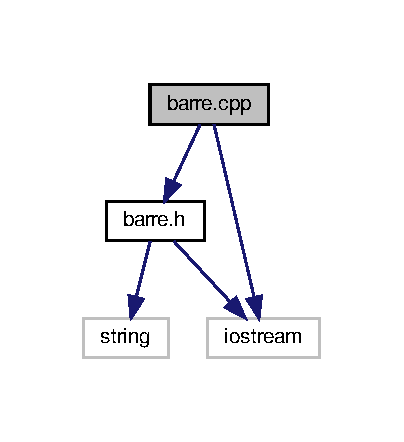
\includegraphics[width=194pt]{barre_8cpp__incl}
\end{center}
\end{figure}

\hypertarget{barre_8h}{}\section{barre.\+h File Reference}
\label{barre_8h}\index{barre.\+h@{barre.\+h}}
{\ttfamily \#include $<$string$>$}\newline
{\ttfamily \#include $<$iostream$>$}\newline
Include dependency graph for barre.\+h\+:
\nopagebreak
\begin{figure}[H]
\begin{center}
\leavevmode
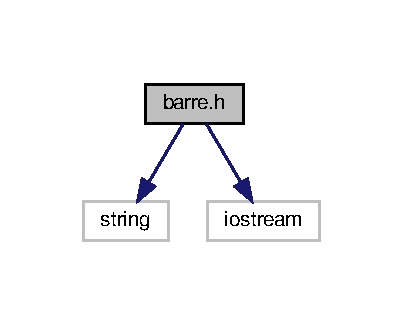
\includegraphics[width=194pt]{barre_8h__incl}
\end{center}
\end{figure}
This graph shows which files directly or indirectly include this file\+:
\nopagebreak
\begin{figure}[H]
\begin{center}
\leavevmode
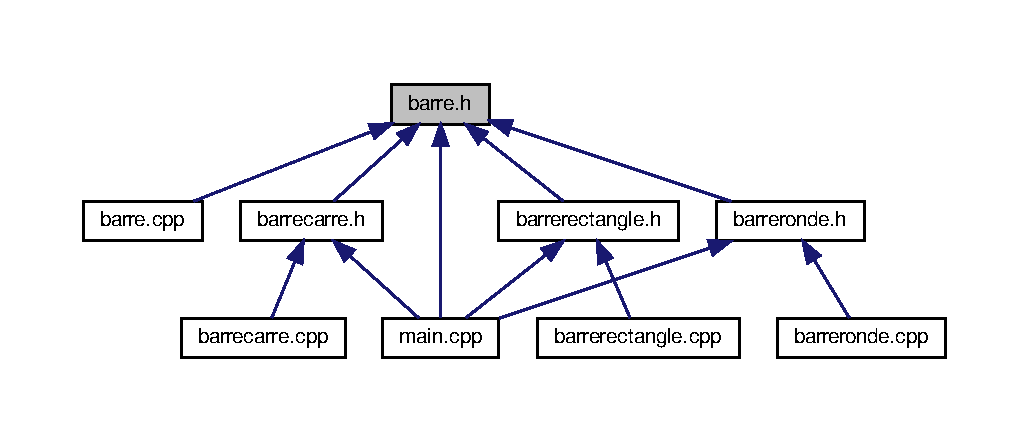
\includegraphics[width=350pt]{barre_8h__dep__incl}
\end{center}
\end{figure}
\subsection*{Classes}
\begin{DoxyCompactItemize}
\item 
class \hyperlink{class_barre}{Barre}
\begin{DoxyCompactList}\small\item\em The \hyperlink{class_barre}{Barre} class. \end{DoxyCompactList}\end{DoxyCompactItemize}

\hypertarget{barrecarre_8cpp}{}\section{barrecarre.\+cpp File Reference}
\label{barrecarre_8cpp}\index{barrecarre.\+cpp@{barrecarre.\+cpp}}
{\ttfamily \#include \char`\"{}barrecarre.\+h\char`\"{}}\newline
Include dependency graph for barrecarre.\+cpp\+:
\nopagebreak
\begin{figure}[H]
\begin{center}
\leavevmode
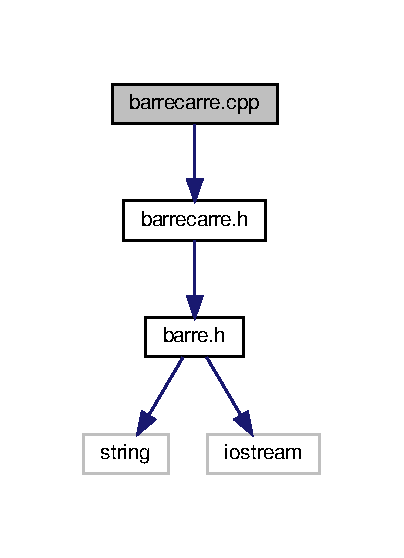
\includegraphics[width=194pt]{barrecarre_8cpp__incl}
\end{center}
\end{figure}

\hypertarget{barrecarre_8h}{}\section{barrecarre.\+h File Reference}
\label{barrecarre_8h}\index{barrecarre.\+h@{barrecarre.\+h}}
{\ttfamily \#include $<$barre.\+h$>$}\newline
Include dependency graph for barrecarre.\+h\+:
\nopagebreak
\begin{figure}[H]
\begin{center}
\leavevmode
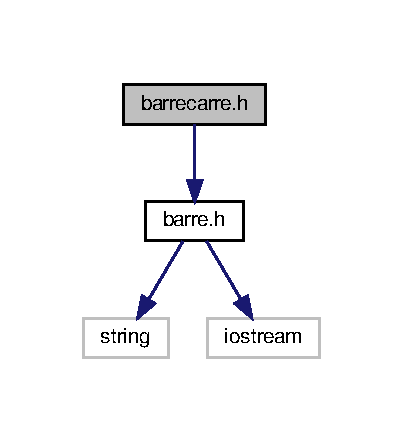
\includegraphics[width=194pt]{barrecarre_8h__incl}
\end{center}
\end{figure}
This graph shows which files directly or indirectly include this file\+:
\nopagebreak
\begin{figure}[H]
\begin{center}
\leavevmode
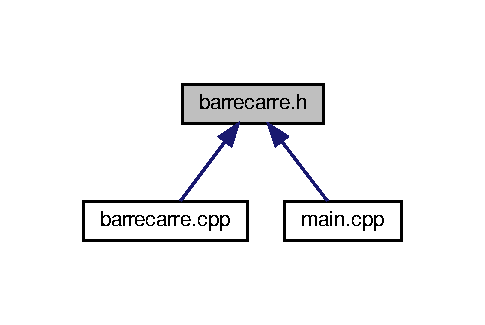
\includegraphics[width=233pt]{barrecarre_8h__dep__incl}
\end{center}
\end{figure}
\subsection*{Classes}
\begin{DoxyCompactItemize}
\item 
class \hyperlink{class_barre_carre}{Barre\+Carre}
\begin{DoxyCompactList}\small\item\em The \hyperlink{class_barre_carre}{Barre\+Carre} class. \end{DoxyCompactList}\end{DoxyCompactItemize}

\hypertarget{barrerectangle_8cpp}{}\section{barrerectangle.\+cpp File Reference}
\label{barrerectangle_8cpp}\index{barrerectangle.\+cpp@{barrerectangle.\+cpp}}
{\ttfamily \#include \char`\"{}barrerectangle.\+h\char`\"{}}\newline
Include dependency graph for barrerectangle.\+cpp\+:
\nopagebreak
\begin{figure}[H]
\begin{center}
\leavevmode
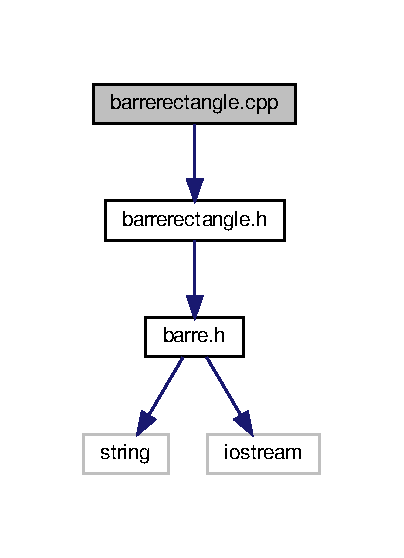
\includegraphics[width=194pt]{barrerectangle_8cpp__incl}
\end{center}
\end{figure}

\hypertarget{barrerectangle_8h}{}\section{barrerectangle.\+h File Reference}
\label{barrerectangle_8h}\index{barrerectangle.\+h@{barrerectangle.\+h}}
{\ttfamily \#include $<$barre.\+h$>$}\newline
Include dependency graph for barrerectangle.\+h\+:
\nopagebreak
\begin{figure}[H]
\begin{center}
\leavevmode
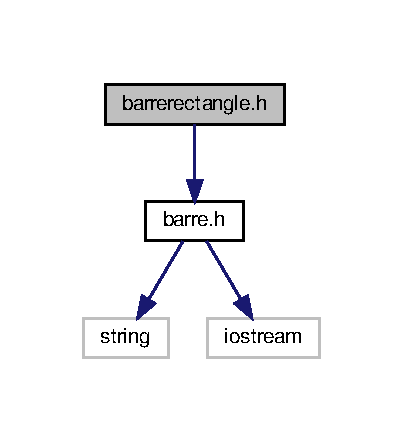
\includegraphics[width=194pt]{barrerectangle_8h__incl}
\end{center}
\end{figure}
This graph shows which files directly or indirectly include this file\+:
\nopagebreak
\begin{figure}[H]
\begin{center}
\leavevmode
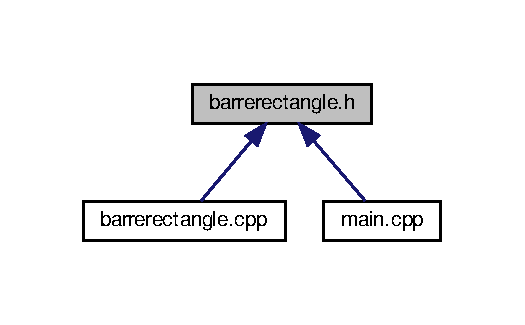
\includegraphics[width=252pt]{barrerectangle_8h__dep__incl}
\end{center}
\end{figure}
\subsection*{Classes}
\begin{DoxyCompactItemize}
\item 
class \hyperlink{class_barre_rectangle}{Barre\+Rectangle}
\begin{DoxyCompactList}\small\item\em The \hyperlink{class_barre_rectangle}{Barre\+Rectangle} class. \end{DoxyCompactList}\end{DoxyCompactItemize}

\hypertarget{barreronde_8cpp}{}\section{barreronde.\+cpp File Reference}
\label{barreronde_8cpp}\index{barreronde.\+cpp@{barreronde.\+cpp}}
{\ttfamily \#include \char`\"{}barreronde.\+h\char`\"{}}\newline
{\ttfamily \#include $<$math.\+h$>$}\newline
Include dependency graph for barreronde.\+cpp\+:
\nopagebreak
\begin{figure}[H]
\begin{center}
\leavevmode
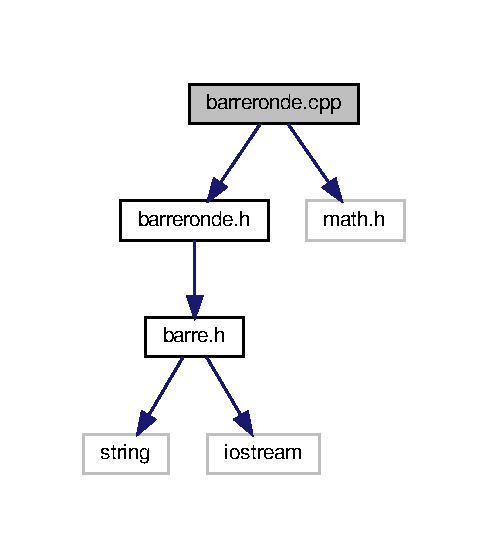
\includegraphics[width=234pt]{barreronde_8cpp__incl}
\end{center}
\end{figure}

\hypertarget{barreronde_8h}{}\section{barreronde.\+h File Reference}
\label{barreronde_8h}\index{barreronde.\+h@{barreronde.\+h}}
{\ttfamily \#include $<$barre.\+h$>$}\newline
Include dependency graph for barreronde.\+h\+:
\nopagebreak
\begin{figure}[H]
\begin{center}
\leavevmode
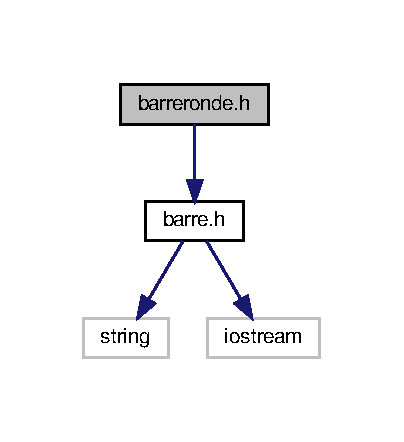
\includegraphics[width=194pt]{barreronde_8h__incl}
\end{center}
\end{figure}
This graph shows which files directly or indirectly include this file\+:
\nopagebreak
\begin{figure}[H]
\begin{center}
\leavevmode
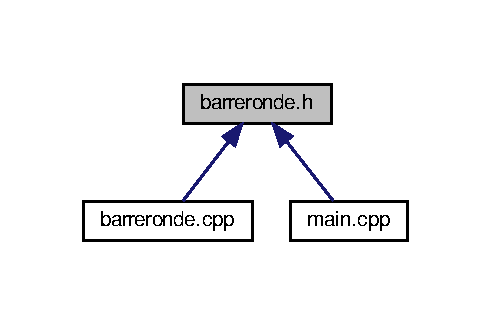
\includegraphics[width=236pt]{barreronde_8h__dep__incl}
\end{center}
\end{figure}
\subsection*{Classes}
\begin{DoxyCompactItemize}
\item 
class \hyperlink{class_barre_ronde}{Barre\+Ronde}
\begin{DoxyCompactList}\small\item\em The \hyperlink{class_barre_ronde}{Barre\+Ronde} class. \end{DoxyCompactList}\end{DoxyCompactItemize}

\hypertarget{main_8cpp}{}\section{main.\+cpp File Reference}
\label{main_8cpp}\index{main.\+cpp@{main.\+cpp}}
{\ttfamily \#include $<$iostream$>$}\newline
{\ttfamily \#include $<$iomanip$>$}\newline
{\ttfamily \#include $<$barre.\+h$>$}\newline
{\ttfamily \#include $<$barreronde.\+h$>$}\newline
{\ttfamily \#include $<$barrerectangle.\+h$>$}\newline
{\ttfamily \#include $<$barrecarre.\+h$>$}\newline
Include dependency graph for main.\+cpp\+:
\nopagebreak
\begin{figure}[H]
\begin{center}
\leavevmode
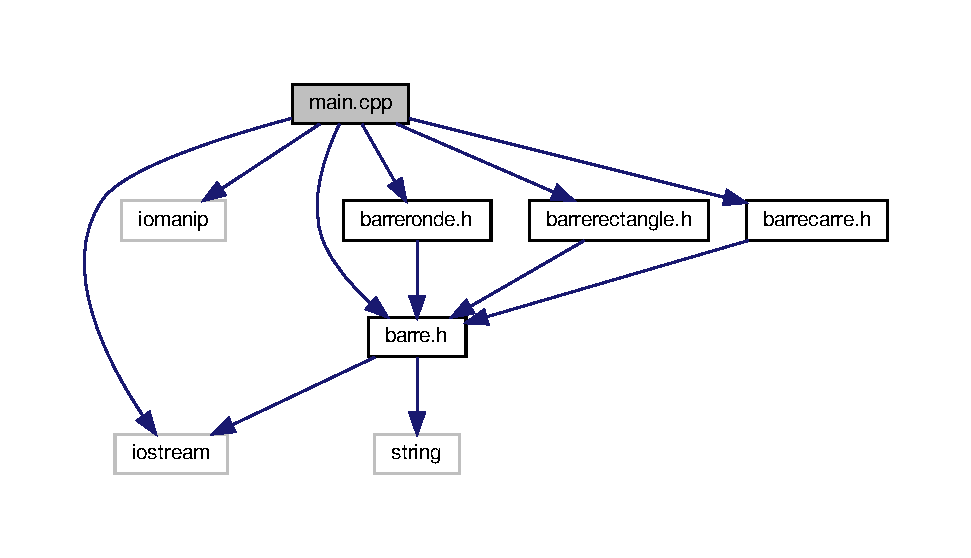
\includegraphics[width=350pt]{main_8cpp__incl}
\end{center}
\end{figure}
\subsection*{Functions}
\begin{DoxyCompactItemize}
\item 
int \hyperlink{main_8cpp_ae66f6b31b5ad750f1fe042a706a4e3d4}{main} ()
\begin{DoxyCompactList}\small\item\em main \end{DoxyCompactList}\end{DoxyCompactItemize}


\subsection{Function Documentation}
\mbox{\Hypertarget{main_8cpp_ae66f6b31b5ad750f1fe042a706a4e3d4}\label{main_8cpp_ae66f6b31b5ad750f1fe042a706a4e3d4}} 
\index{main.\+cpp@{main.\+cpp}!main@{main}}
\index{main@{main}!main.\+cpp@{main.\+cpp}}
\subsubsection{\texorpdfstring{main()}{main()}}
{\footnotesize\ttfamily int main (\begin{DoxyParamCaption}{ }\end{DoxyParamCaption})}



main 

Affiche les caratéristque de la barre et affiche les sections et les masse des differents type de barre en fonction de la barre \begin{DoxyReturn}{Returns}

\end{DoxyReturn}

%--- End generated contents ---

% Index
\backmatter
\newpage
\phantomsection
\clearemptydoublepage
\addcontentsline{toc}{chapter}{Index}
\printindex

\end{document}
